\documentclass[conference]{IEEEtran}
\usepackage{graphicx}
\usepackage{listings}
\usepackage{hyperref}

\hypersetup{
    colorlinks=true,
    linkcolor=blue,
    filecolor=magenta,      
    urlcolor=cyan,
}

\begin{document}

\title{AURO REPORT}
\author{\IEEEauthorblockN{Module Code: COM00052H | Examination Number: Y3898642}}

\maketitle

%\section{Assessment Introduction}
%For this assessment, we've been tasked with programming autonomous mobile robots, specifically the TurtleBot3 Waffle Pi, to navigate through a simulated environment with obstacles, and retrieve items scattered around before returning them to the home zone.

\section{Design}
\subsection{System Overview}
In the design of my autonomous robot, I implemented a modular approach with the TurtleBot3, using the ROS2 framework. At the heart of the design is a finite state machine (FSM), which contains the robot's states - FORWARD, TURNING, COLLECTING, and RETURNING. This FSM was chosen for its ability to provide structured yet flexible control, which is essential for navigation and adapting to dynamic task requirements. The keys to perception were the LiDAR and camera sensors, which are essential for effective operation. Their integration within ROS2 is indispensable for the task.

\begin{figure}[htbp]
\centerline{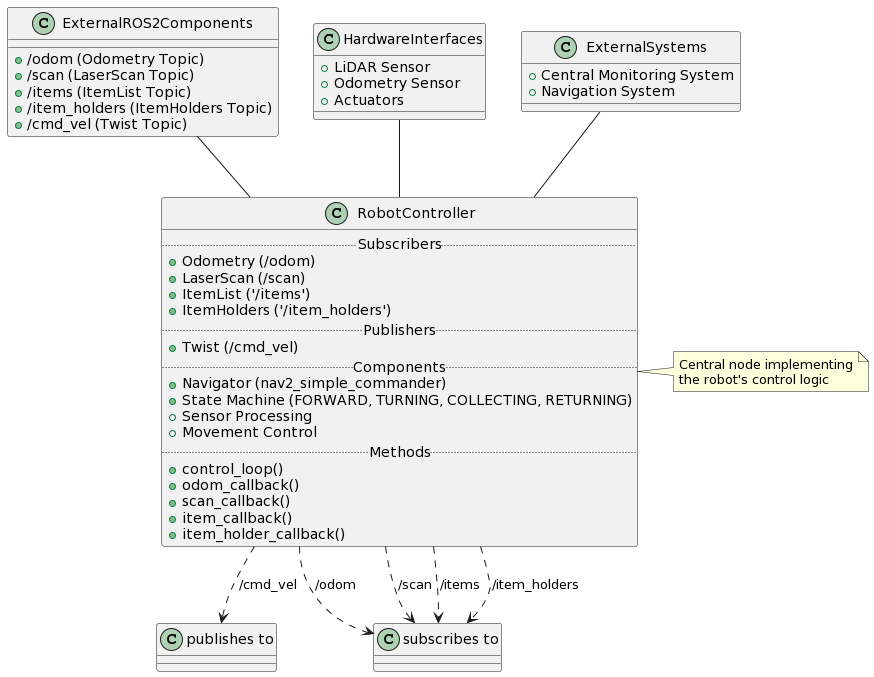
\includegraphics[width=\linewidth]{high-level system diagram.png}}
\caption{High-Level System Design}
\label{fig:systemdesign}
\end{figure}

\subsection{Component Interaction}
As shown in Fig.~\ref{fig:systemdesign}, the robot controller subscribes to several essential topics for efficient operation:

\begin{itemize}
    \item \textbf{LaserScan}: Provides obstacle navigation data, taken from the LiDAR sensor, enabling the robot to detect and avoid obstacles.
    \item \textbf{ItemList}: Processes information from the camera to identify items within the robot's field of view, facilitating item identification and retrieval.
    \item \textbf{ItemHolders}: Keeps track of the items held by each robot, sourced from internal status monitoring. Helps in preventing task ovelap.
    \item \textbf{Odometry}: Provides data on the robot's position and orientation, taken from odometry sensors. It's essential for accurate navigation and precise maneuvering.
\end{itemize}

The data from these topics is parsed using the callback methods, a key process in the system's functionality.

\section{Implementation}
\subsection{ROS Architecture}
The implementation of my autonomous robot system is deeply rooted in the ROS 2 framework. It provides a modular and scalable architecture. This architecture is made from multiple ROS 2 nodes, each of which performs specific functions such as sensor data processing, state management, and motion control. The communication among these nodes is facilitated through topics, in which nodes publish and subscribe to messages.

\subsection{Node Structure and Topic Communication}
The system is structured around several key nodes. For example, the \texttt{robot\_controller} node subscribes to the \texttt{/scan} topic for LiDAR data and the \texttt{/odom} topic for odometry information. It also publishes movement commands to the \texttt{/cmd\_vel} topic.

\begin{figure}[htbp]
\centerline{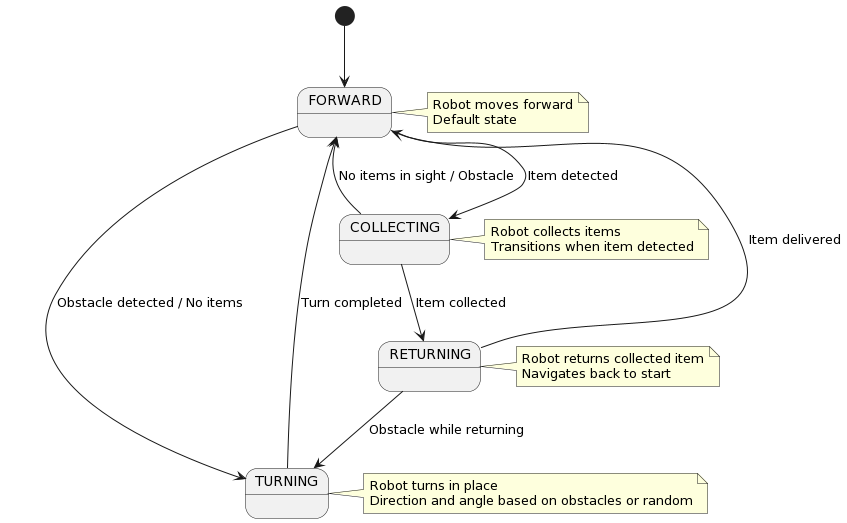
\includegraphics[width=\linewidth]{statediagram.png}}
\caption{Finite State Machine Representing Autonomy}
\label{fig:statemachine}
\end{figure}

\subsection{Autonomy Realization}
Autonomy in the system is achieved through a well-defined finite state machine (FSM), as depicted in Fig.~\ref{fig:statemachine}. The FSM has 4 states in which it can be: FORWARD, TURNING, COLLECTING, and RETURNING. It transitions based on sensor inputs and internal logic, also shown in Fig.~\ref{fig:statemachine}.

\subsection{Sensor Integration and Data Processing}
Integrating sensors like LiDAR and cameras is key to the robot's perception capabilities. Using ROS 2, sensor data is processed in real-time, with custom callback functions handling the data for tasks like obstacle detection and item identification. Without this processed information, navigation decisions and effective task execution would be impossible.

\subsection{Actuation and Movement Control}
Movement control within the system is made through the generation of Twist messages. Those messages determine the robot's linear and angular velocities, and are based on the current state of the FSM and the processed sensor data. This shows a direct link between sensory input and actuator output.

\subsection{Challenges and Solutions}
During the early phases of the development process, I started with designing and implementing a system for a single robot. This approach, however, later caused issues whilst integrating the multi-robot solution. One such issue was all robots transitioning to the RETURNING state once one of them collected an item. This was due to the lack of optimisation for a multi-robot system. For instance, the \texttt{item\_holder\_callback} method was returning all the bots' information simultaneously, which caused the issue. The solution was to ensure each robot received and acted upon only the information relevant to itself. This change made the system effectively manage the state transitions for each robot independently and further align with the demands of a multi-robot system.

\section{Analysis}
\subsection{Experimental Approach}

To evaluate the performance and efficiency of the system, I've taken a comprehensive experimental approach. This involved multiple strategies to gather both qualitative and quantitative data:
\begin{itemize}
    \item \textbf{Data Logging}: Extensive data logging into the terminal was performed to capture real-time operational details of the system - This helped find bugs and solve issues.
    \item \textbf{Visual Inspections}: During simulations, visual inspections / Analysis were done to identify and fix issues in the system's behavior.
    \item \textbf{Simulation Analysis}: Detailed analysis of data logs from 10 different simulations, each lasting 5 minutes in real-time (approximately 1:30 - 2:00 minutes in simulation time in my environment). These simulations each used different item manager 'seeds' to assess the system's efficiency and adaptability under different conditions.
\end{itemize}
Repeated trials were also conducted to ensure the reliability and consistency of the system’s performance across various scenarios.


\subsection{Results}
The results of the experiments are presented in Fig.~\ref{fig:performancegraph} and Table~\ref{tab:performance}. 

\begin{figure}[htbp]
\centerline{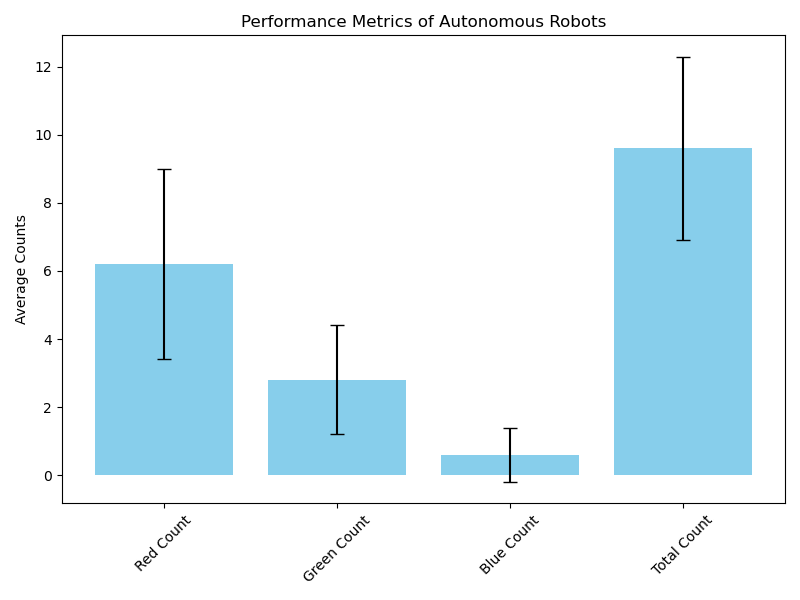
\includegraphics[width=\linewidth]{performance_metrics.png}}
\caption{Bar-Plot Showcasing Performance }
\label{fig:performancegraph}
\end{figure}

\begin{table}[htbp]
\caption{Performance Metrics}
\begin{center}
\begin{tabular}{|c|c|c|}
\hline
Metric & Average & Standard Deviation \\
\hline
Red Count & 6.2 & 2.79 \\
Green Count & 2.8 & 1.60 \\
Blue Count & 0.6 & 0.80 \\
Total Count & 9.6 & 2.69 \\
\hline
\end{tabular}
\label{tab:performance}
\end{center}
\end{table}

\subsection{Results Analysis}

Qualitatively, the system showed decent performance in item collection, with an average of approximately 10 items per simulation. Notably, red items were collected most frequently, as they were positioned closest to the home zone. Green items, typically located in the middle, were collected next in frequency, followed by blue items, which were the furthest away. Despite the robots being programmed to prioritize blue, then green, and then red items within their field of view when collecting, this priority order does not reflect itself in the results.

Quantitatively, the reason behind this can be understood through the visual inspections conducted during the simulations. While the robots initially prioritize blue items, they often collect green or red items en route to the blue ones, leading them to transition to the returning state prematurely. Additionally, on their way back to the home zone with a blue or green item, they frequently swap it for more readily accessible red items. This behavior is linked to the functionality of the item manager, though it is unclear whether this is a bug or an intentional design choice. An alternative approach could have been to treat untargeted items as obstacles when the robot is in the returning state, which would prevent item swapping. Doing so would result in a higher count of blue and green items, however, it would also increase the time taken for the robot to return home, decreasing the total count of collected items.

\section{Evaluation}
\subsection{Strengths and Weaknesses}

During the development and testing phase, several strengths and weaknesses in the system became evident. One key strength is the design's scalability and adaptability which allowed for a smooth integration of multi-robots, capable of efficiently handling multiple tasks such as navigation, item collection and obstacle avoidance. The implementation of the FSM, shown in Fig.~\ref{fig:statemachine}, was crucial for the system, significantly contributing to its operational success.

On the flip side, weaknesses were also shown in the system, especially in the context of multi-robot coordination. Notably, in rare cases, robots attempted to collect items already held by another. This behaviour stems from an oversight in the COLLECTING state's logic, which doesn't account for other robots' activities. An easy potential fix could involve considering the y-coordinate of the item; since the ground is always level in the simulation, items at a higher y-coordinate are likely being held by another robot. However, this solution might not be feasible in a more complex real-world environment with varying elevations.

Improving the system further could involve advancing the communication between robots. By sharing their current positions and the status of items they're carrying, each robot would be aware of its peers' activities. This enhancement, integrated within the ROS2 framework, would make the system even more efficient, and address a big chunk of its weaknesses.

\subsection{Transferability to Reality}
When considering the transfer of the autonomous robot system from simulation to real-world scenarios, several key factors come into play. The simulation provides a controlled environment which significantly differs from the real-world, which can be unpredictable due to the varied terrain, unexpected obstacles, and hardware issues (especially with sensors).

The TurtleBot3's modular design and the ROS2 framework provides a good starting point for this transition, however, adapting the system for real-world use would require additional enhancements such as:

\begin{itemize}
    \item \textbf{Enhanced Sensor data processing}: To deal with faults, and handle errors.
    \item \textbf{Enhanced Navigation Algorithms}: To handle more complex and less predictable environments.
    \item \textbf{Enhanced Obstacle Avoidance}: Since you can't walk through items in real life, they have to be treated as obstacles.
    \item \textbf{Addition of Robot Arm}: To grab and hold the items, since they don't magically get on the robot like in the simulation.
\end{itemize}

More challenges and unforeseen issues can occur in real-world applications, it would require more development and testing to fully know what's needed.

\section{Safety and Ethics}
The integration of autonomous robots into real-world scenarios, especially for tasks such as item retrieval, brings forth significant safety implications and ethical considerations.

\subsection{Safety Considerations}
The safety of both the robots and humans they may interact with is crucial. For this reason, designing fail-safes and emergency stop mechanisms to prevent accidents is necessary. 
A robot might malfunction and run into a human (could stem from sensor malfunction, detects human as an item and tries to retrieve it), which could cause damage to both parties involved.
The robots might malfunction and run into each other, or into obstacles. This might cause damage to the robots, and environment surrounding them. Later resulting in injuries and financial loss.  

\subsection{Ethical Considerations}
Ethically, it's crucial to consider the potential impact of these robots on human employment and privacy, especially in contexts where they operate in close proximity to people.
Data collected from the robots might have an impact on people's privacy. Camera data, could potentially be used for facial recognition and be later sold to companies, profiting from non-consenting humans is ethically wrong. This could be solved by making sure all data stemmed from the robots is used in an ethical way, and was gathered with consent from all parties involved.
The deployment of such systems should be guided by principles that prioritize human welfare, and job security. Doing so ensures that the technology augments human roles, not replace them.

\section{Conclusion}
This report has presented the design, implementation, analysis, and evaluation of an autonomous robot system using the TurtleBot3 Waffle Pi and the ROS2 framework. The system, structured around a finite state machine (FSA), demonstrated strengths in scalability, adaptability, and the capability to handle multiple tasks like navigation, item collection, and obstacle avoidance, as shown in the analysis section.

Key findings from the project include:
\begin{itemize}
    \item The modular design approach facilitated efficient multi-robot integration and task management.
    \item The implementation of the FSM was instrumental in achieving autonomous operations, despite some challenges in multi-robot coordination.
    \item Experimental analysis highlighted the system’s proficiency in item retrieval, with some limitations noted in prioritizing specific items due to the current item management strategy.
    \item Safety and ethical considerations underscored the need for robust design, including fail-safes and privacy safeguards, particularly for real-world applications.
\end{itemize}

Future work for improving the system could focus on several areas such as:
\begin{itemize}
    \item Enhancing inter-robot communication to optimize task allocation and prevent redundant efforts in item collection.
    \item Refining sensor integration and data processing techniques to better handle real-world environments.
    \item Integrating a robot arm for physical item retrieval in real-world scenarios.
    \item Addressing the ethical implications of autonomous robotics, ensuring that the technology serves to augment human efforts rather than replace them.
\end{itemize}

Continued development and testing in a variety of environments will be essential to prepare the system for real-world deployment. This is to ensure its reliability, safety, and ethical compliance. The knowledge gained from this project will lay a strong foundation for further advancements in the field of autonomous robotics.


\bibliographystyle{IEEEtran}
\bibliography{references}

\end{document}

%Describe your approach to experimental analysis.

%To evaluate the performance and efficiency of the system, I've taken a comprehensive experimental approach. The approaches were: logging data into the terminal, visually looking for problems while the simulations were running, and analyzing data logs from 10 different simulations (5 minutes each real time, 1:30 minutes roughly simulation time, different item distribution "seeds" were used in each simulation). Repeated trials were performed to ensure the reliability of the system.

%To evaluate the performance and efficiency of the system, I've taken a comprehensive experimental approach. This involved a multiple strategies to gather both qualitative and quantitative data. Firstly, extensive data logging into the terminal was performed to capture real-time operational details. Secondly, visual inspections were conducted during simulations to identify any immediate issues in the system's behavior. Finally, detailed analyses were carried out on data logs from 10 different simulations, each lasting 5 minutes in real-time (approximately 1:30 minutes in simulation time in my environment). These simulations were varied using different item distribution 'seeds' to test the system's robustness and adaptability under diverse conditions. Repeated trials ensured the reliability and consistency of the system’s performance across various scenarios.

%Qualitatively, the system demonstrated decent results for collecting the items with a rounded average of 10 items per simulation. The red items were the most collected due to them being the closest to the home zone, green after due to them being mostly in the middle, and blue in last due to them being the furthest away. The robots are programmed to prioritise blue, then green then red items within its FOV when going to collect but this doesnt show in the results, let's see why.

%Quantitavely, this can be explained thanks to the visual inspections done during the simulations. Whilst the robots prioritise the blue items, they end up picking up green / red items on their way to getting the blue ones, thus transitioning to return state. Or if they reach the blue ones, they transition to returning state, they end up swapping the held item (in this scenario blue items) with other colored items (mostly reds cuz theyre the closest to the home) when they're driving back home. The items are swapped because thats how the item manager is made, unsure if its a bug or intentional. Could've treated the items as obstacles when robot is in return state (holding an item) but that would result in the robot taking too much time to return and would result in the total count average dropping quite a bit. but would result in more blue and green items overall.

%\section{Evaluation}
%Discuss the strengths and weaknesses of your solution based on your design, implementation, and analysis. Address the transferability of your solution from simulation to reality.
%During the development and testing phase, several strengths and weaknesses in the system became evident. One key strength would be the design; it allowed for multi-robot integration without much problems. It's scalable, adaptable and capable of efficiently handling multiple tasks such as navigation, item collection and obstacle avoidance. Implementing the FSM shown in Fig.~\ref{fig:statemachine}. was crucial for the system, and allowed it to perform the way it does.

%On the flip side, the system also showed some weaknesses, particularly in the context of multi-robot coordination. In rare cases, the robots tries to collect items held by another robot returning home. This is due to an oversight in the internal logic of the COLLECTING state, which doesn't account for another robot holding an item. In context of this assessment, an easy fix could be taking the y value of an item into account. Since the ground is level and there are no elevations, an item with a higher y coordinate would mean it's being held by another robot. However, this fix wouldn't transfer well to reality. Better communication between the robots so they know who is holding what item and where they are on the map

%In terms of transferability to real-world scenarios, the system's reliance on accurate sensor data and the efficiency of its state transition logic are critical factors. While the simulation provides a controlled environment to test these aspects, real-world conditions often introduce complexities such as dynamic obstacles, variable lighting, and sensor noise. Addressing these challenges would require additional layers of complexity in the system's design and implementation, such as advanced sensor fusion techniques and more sophisticated decision-making algorithms to handle unpredictable environments.

%Furthermore, the mechanical and hardware limitations of the TurtleBot3 platform in real-world applications, such as battery life and terrain handling capabilities, must also be considered for a successful transition from simulation to reality.